% This is file NWSguide.tex
% release v1.00, 12th June 2012
%   (based on JFPguide.tex v1.11 for LaTeX 2.09)
% Copyright (C) 2012 Cambridge University Press

\NeedsTeXFormat{LaTeX2e}

\documentclass{nws}

%%% Macros for the guide only %%%
\providecommand\AMSLaTeX{AMS\,\LaTeX}
\newcommand\eg{\emph{e.g.}\ }
\newcommand\etc{\emph{etc.}}
\newcommand\bcmdtab{\noindent\bgroup\tabcolsep=0pt%
  \begin{tabular}{@{}p{10pc}@{}p{20pc}@{}}}
\newcommand\ecmdtab{\end{tabular}\egroup}
\newcommand\rch[1]{$\longrightarrow\rlap{$#1$}$\hspace{1em}}
\newcommand\lra{\ensuremath{\quad\longrightarrow\quad}}

\title[Measures of Topic Centrality for Online Political Engagement]
      {Measures of Topic Centrality for Online Political Engagement}

 \author[C.J.K Raymond]
        {Cameron Raymond\\
        School of Computing, Queen's University, Kingston K7L 3N6, CA\\
         \email{c.raymond@queensu.ca}}

\jdate{May 2020}
\pubyear{2020}
\pagerange{\pageref{firstpage}--\pageref{lastpage}}
% \doi{S0956796801004857}

% \newtheorem{lemma}{Lemma}[section]

\begin{document}

\label{firstpage}

\maketitle

\begin{abstract}
  The advent of social media has enabled political parties to engage with the
  broader populous in new and unforeseen ways -- and the ability to bypass the
  traditional mediating forces of mass media allows for an unfiltered promotion
  of policy, ideology and party stances. Drawing on Twitter data leading up to
  the 2019 Canadian Federal Election, this paper develops two novel, graph-based methods that
  capture how different categories of messages drive different patterns of political
  engagement. Through the two proposed variations of topic centrality -- on which
  measures how central a topic was to the general discourse, and one which
  measures how central a topic was to a particular voting bloc -- statistically
  significant variations in topic centrality are then shown and discussed. %MORE_SPECIFIC
  \paragraph{Keywords:} \emph{centrality, political communication, social media, topic modeling}
\end{abstract}

\tableofcontents

\section{Introduction}

The way information is distributed and received has changed significantly over
the past decade. As Cogburn and Espinoza-Vasquez argue, Barrack Obama’s 2008
presidential campaign was a watershed moment in social media campaigning – and
in the subsequent decade, from Macron to Brexit to the Five Star Movement,
social media has played an increasing role in how politics is conducted
\cite{cogburn2011networked}.  The same holds true for Canada, between 2013 and
2018 the share of Canadian federal media expenditure spent on digital
advertising rose from 27\% to 65\%, a 140\% increase, making the study of new
media critical from a social science perspective
\cite{annualReportCanadaAdvertisingActivities_2018}. Over the past 12 years,
political elites have subverted traditional models of political communication by
using social media to directly promote various policies, topics and issues to
the electorate\footnote{The
terms policy, issue and topic will be used interchangeably to refer to
categories of messages.}\cite{mcnair2017introduction}.

Additionally, it is important to note that not all messages promoted by
political elites are likely to serve the same purpose. Some topics may be
logistical in nature, informing party affiliates of campaign events; other
topics may be promoted in an attempt to rally that party's core voting bloc;
others, finally, may be an attempt to attract
engagement from new, untapped demographics. The latter two categories are in
many ways analogous to Robert Putnam's conception of social capital
\cite{putnam2001social}. Here, Putnam draws the distinction between two forms
of social capital: bonding social capital, which occurs within a group -- and
bridging social capital, which unites different demographics
\cite{putnam2001social}. Therefore, the research question being proposed is:
are their data to support the notion that some political messages are bonding in
nature, rallying members within a group, while other political messages are
bridging in nature? This question will be answered within the context of the
2019 Canadian Federal Election with the Tweets of Canada’s five major, english
speaking party leaders: Andrew Scheer, Elizabeth May, Jagmeet Singh, Justin
Trudeau, and Maxime Bernier. 

In order to answer this question, a justification of Canadian politics and
social media data in this context will be given. Then an overview of the data
collected and a formal definition of the political engagement graph used will
allow for the exploration of two measures of topic centrality: total network
topic centrality, and party leader topic centrality. Finally, results from this
process and a discussion of their implications will highlight possibilities for
future research.  

\subsection{Social Media in the Canadian Context}

While it is clear that technology is changing how information is received, and
thus also changing how politics is conducted, it may not be clear the role of
Canadian politics in this context. However, Canada’s political system is a
fertile environment to test the importance of political messaging, because
relative to most liberal democracies, it is dominated by party
politicians. As Carty put it: 

\begin{quote}
  No obvious simple geographic reality, no common linguistic or religious
  homogeneity, no common revolutionary experience or unique historical moment
  animated [Canada] or gave it life. Canada was created when a coalition of party
  politicians deemed it to be in their interest to do so, and it has been
  continuously grown, reshaped and defended by its politicians.\cite{carty2010political}
\end{quote}

Thus, it is not surprising that Canada’s electoral system
encourages electoral pragmatism – and developed large, ``big tent'' parties that
are among the most organizationally weak and decentralized of established
democracies \cite{carty2010political}. This system defines political parties as brokers of the often
conflicting, weakly integrated electorate –- as opposed to mobilizers of
distinct communities, articulating claims rooted in their pre-existing
interests. In this way, parties act as the ``principal instruments of national
accommodation, rather than democratic division'' \cite{carty2010political}.

The dominance of parties in Canadian politics, their amorphous ideological
stances, and the many intersectional geographic, linguistic and religious
cleavages have given birth to what’s been coined the brokerage party system
\cite{carty2010political}. The need to capture pluralities in a diverse range of
electoral districts means that most parties have to take stances on most issues,
and thus when a user engages with a specific issue, it doesn’t necessarily
invoke a specific party or vice versa. 

Given the utility of Canadian politics in answering questions about different
axes of political engagement, the question then is: how do we observe these
phenomena? Social media data, culled from platforms like Twitter, are inherently
relational -- and thus lend themselves well to being represented as graphs. An
empirical analysis that observes and measures how users behave and engage with
political parties online privileges this relational aspect of social media.
Social network analysis helps avoid the pitfalls of survey data, famously
described by Allen Barton as “a sociological meat grinder, tearing the
individual from [their] social context” \cite{freeman2004development}.  


\section{Methods}

\subsection{Data}

% Twitter data - %'s and stuff + ReTweet/Tweet graphs
The novel dataset used was collected via Twitter's historical search application
programming interface (API), which allows user's to programmatically access any
publicly available Tweet. The API was used to collect all of the
English\footnote{Denoted by a language marker in the historical search API.}
tweets from Canada's five, english speaking party leaders: Andrew Scheer,
Elizabeth May, Jagmeet Singh, Justin Trudeau, and Maxime Bernier. The timeframe
of collection ranges from October 21, 2018 to October 21, 2019 -- the eve of
Canada’s federal election. While the Tweets from each Federal party’s official
Twitter accounts were also collected, they predominantly acted as logistical
tools – informing party affiliates of events and rallies. The personal accounts
for party leaders were generally more pertinent to their beliefs, platforms and
style of rhetoric, and thus are better suited do analyze the bridging versus
bonding nature of various topics. In this spirit, only Tweets of the party
leader were used, excluding Retweets. Figure \ref{fig:tweets_over_time}
visualizes the daily and cumulative number of Tweets over time, in aggregate and
by party leader, resulting in 7,978 total Tweets. Additionally, for each tweet collected from a party leader, all of the available
Retweets by general users\footnote{The term general users will denote those
active on Twitter who are not party leaders.} were collected for a total of
113,293 Retweets by 36,450 general users. This is, again, visualized in
aggregate and by party leader in Figure \ref{fig:retweets_over_time}.

\begin{figure}[h!]
  \centering
  \includegraphics[width=0.8\textwidth]{figures/tweets_over_time}
  \caption[Daily and Cumulative Tweets over Time]{Daily and Cumulative Tweets over Time}
  \label{fig:tweets_over_time}
\end{figure}

\begin{figure}[h!]
  \centering
  \includegraphics[width=0.8\textwidth]{figures/retweets_over_time}
  \caption[Daily and Cumulative Retweets over Time]{Daily and Cumulative Retweets over Time}
  \label{fig:retweets_over_time}
\end{figure}

Additionally, given the inherent noise and extraneous info in text data, it is
standard and necessary to preprocess text before modeling
\cite{sapul2017trending}. The text cleaning pipeline removes punctuation marks,
stop words, words with fewer than three characters, and URLs, as well as common
Twitter symbols like ``RT:'', ``@'' and ``\#''. Emojis were converted to text
using the python package \texttt{emoji}. After this process, all text was
converted to lower-case and lemmatized to get rid of common suffixes. Therefore,
the tweet in Figure \ref{fig:tweet_ex} after preprocessing reads: \emph{wherever
maple leaf fly represents rich history bright future value hold dear happy flag
day canada}.

\begin{figure}[h!]
  \centering
  \includegraphics[width=0.8\textwidth]{figures/tweet_ex}
  \caption[Daily and Cumulative Retweets over Time]{Daily and Cumulative Retweets over Time}
  \label{fig:tweet_ex}
\end{figure}

\subsubsection{Engagement Graph}

The networks considered in this paper are assumed to be connected, unweighted,
and undirected. Let $(V,E)$ be a network, where $V$ is the set of vertices and
$E$ is the set of edges. If vertex $v_1$ is connected to vertex $v_2$, it is
denoted by $(v_1,v_2)\in E$. Engagement graph's are defined with additional
constraints that denote three categories of vertices: those that \emph{produce
objects} (Tweets, songs, goods, services, etc\dots), those that represent the
objects produced, and a third set of vertices that chooses to engage with the
various produced objects in the network. In this context the engagement graph
represents the Tweets that party leaders produce, and the general users who
choose which Tweets to Retweet. An example of this type of political engagement
graph is shown in figure \ref{fig:ex_engagement_graph}. More formally the
political engagement graph is defined below:

\begin{itemize}
  \item \emph{Vertices}: Let $V_{1}=\{v_{1},v_{2},...,v_{n}\}$ be the set of
  party leaders; $V_{2}=\{v_{1},v_{2},...,v_{m}\}$ be the set of Tweets by the
  party leaders; and let
  $V_{3}=\{v_{1},v_{2},...,v_{k}\}$ be the set of ``general users'' who
  Retweet Tweets. Let the total set of vertices $V=V_{1}\cup V_{2}\cup V_{3}$.
  
  \item \emph{Edges}: Let $E$ be the set of edges. Allow the edge $(v_{1},
  v_{2})\in E$ if and only if $v_{1}\in V_{1}, v_{2}\in V_{2}$ or $v_{1}\in
  V_{3}, v_{2}\in V_{2}$. By this definition, we will only allow edges from a
  party leader vertex to a tweet vertex, or from a generic user vertex to a
  tweet vertex.
\end{itemize}

\begin{figure}[h!]
  \centering
  \includegraphics[scale=0.2]{figures/ex_engagement_graph}
  \caption[Example Engagement Graph]{Example Engagement Graph}
  \label{fig:ex_engagement_graph}
\end{figure}

Further nuances can be added to distinguish between different types of objects,
which in this context would refer to Tweets of different topics. Figure
\ref{fig:engagement_graph_no_topics}  visualizes the full political engagement
graph collected with all 5 party leaders, 7,978 Tweets, 36,450 general users,
and 113,293 Retweets\footnote{The number of Retweets is equivalent to the number
of edges from Tweet vertices to general user vertices.} built with these constraints.

\begin{figure}[h!]
  \centering
  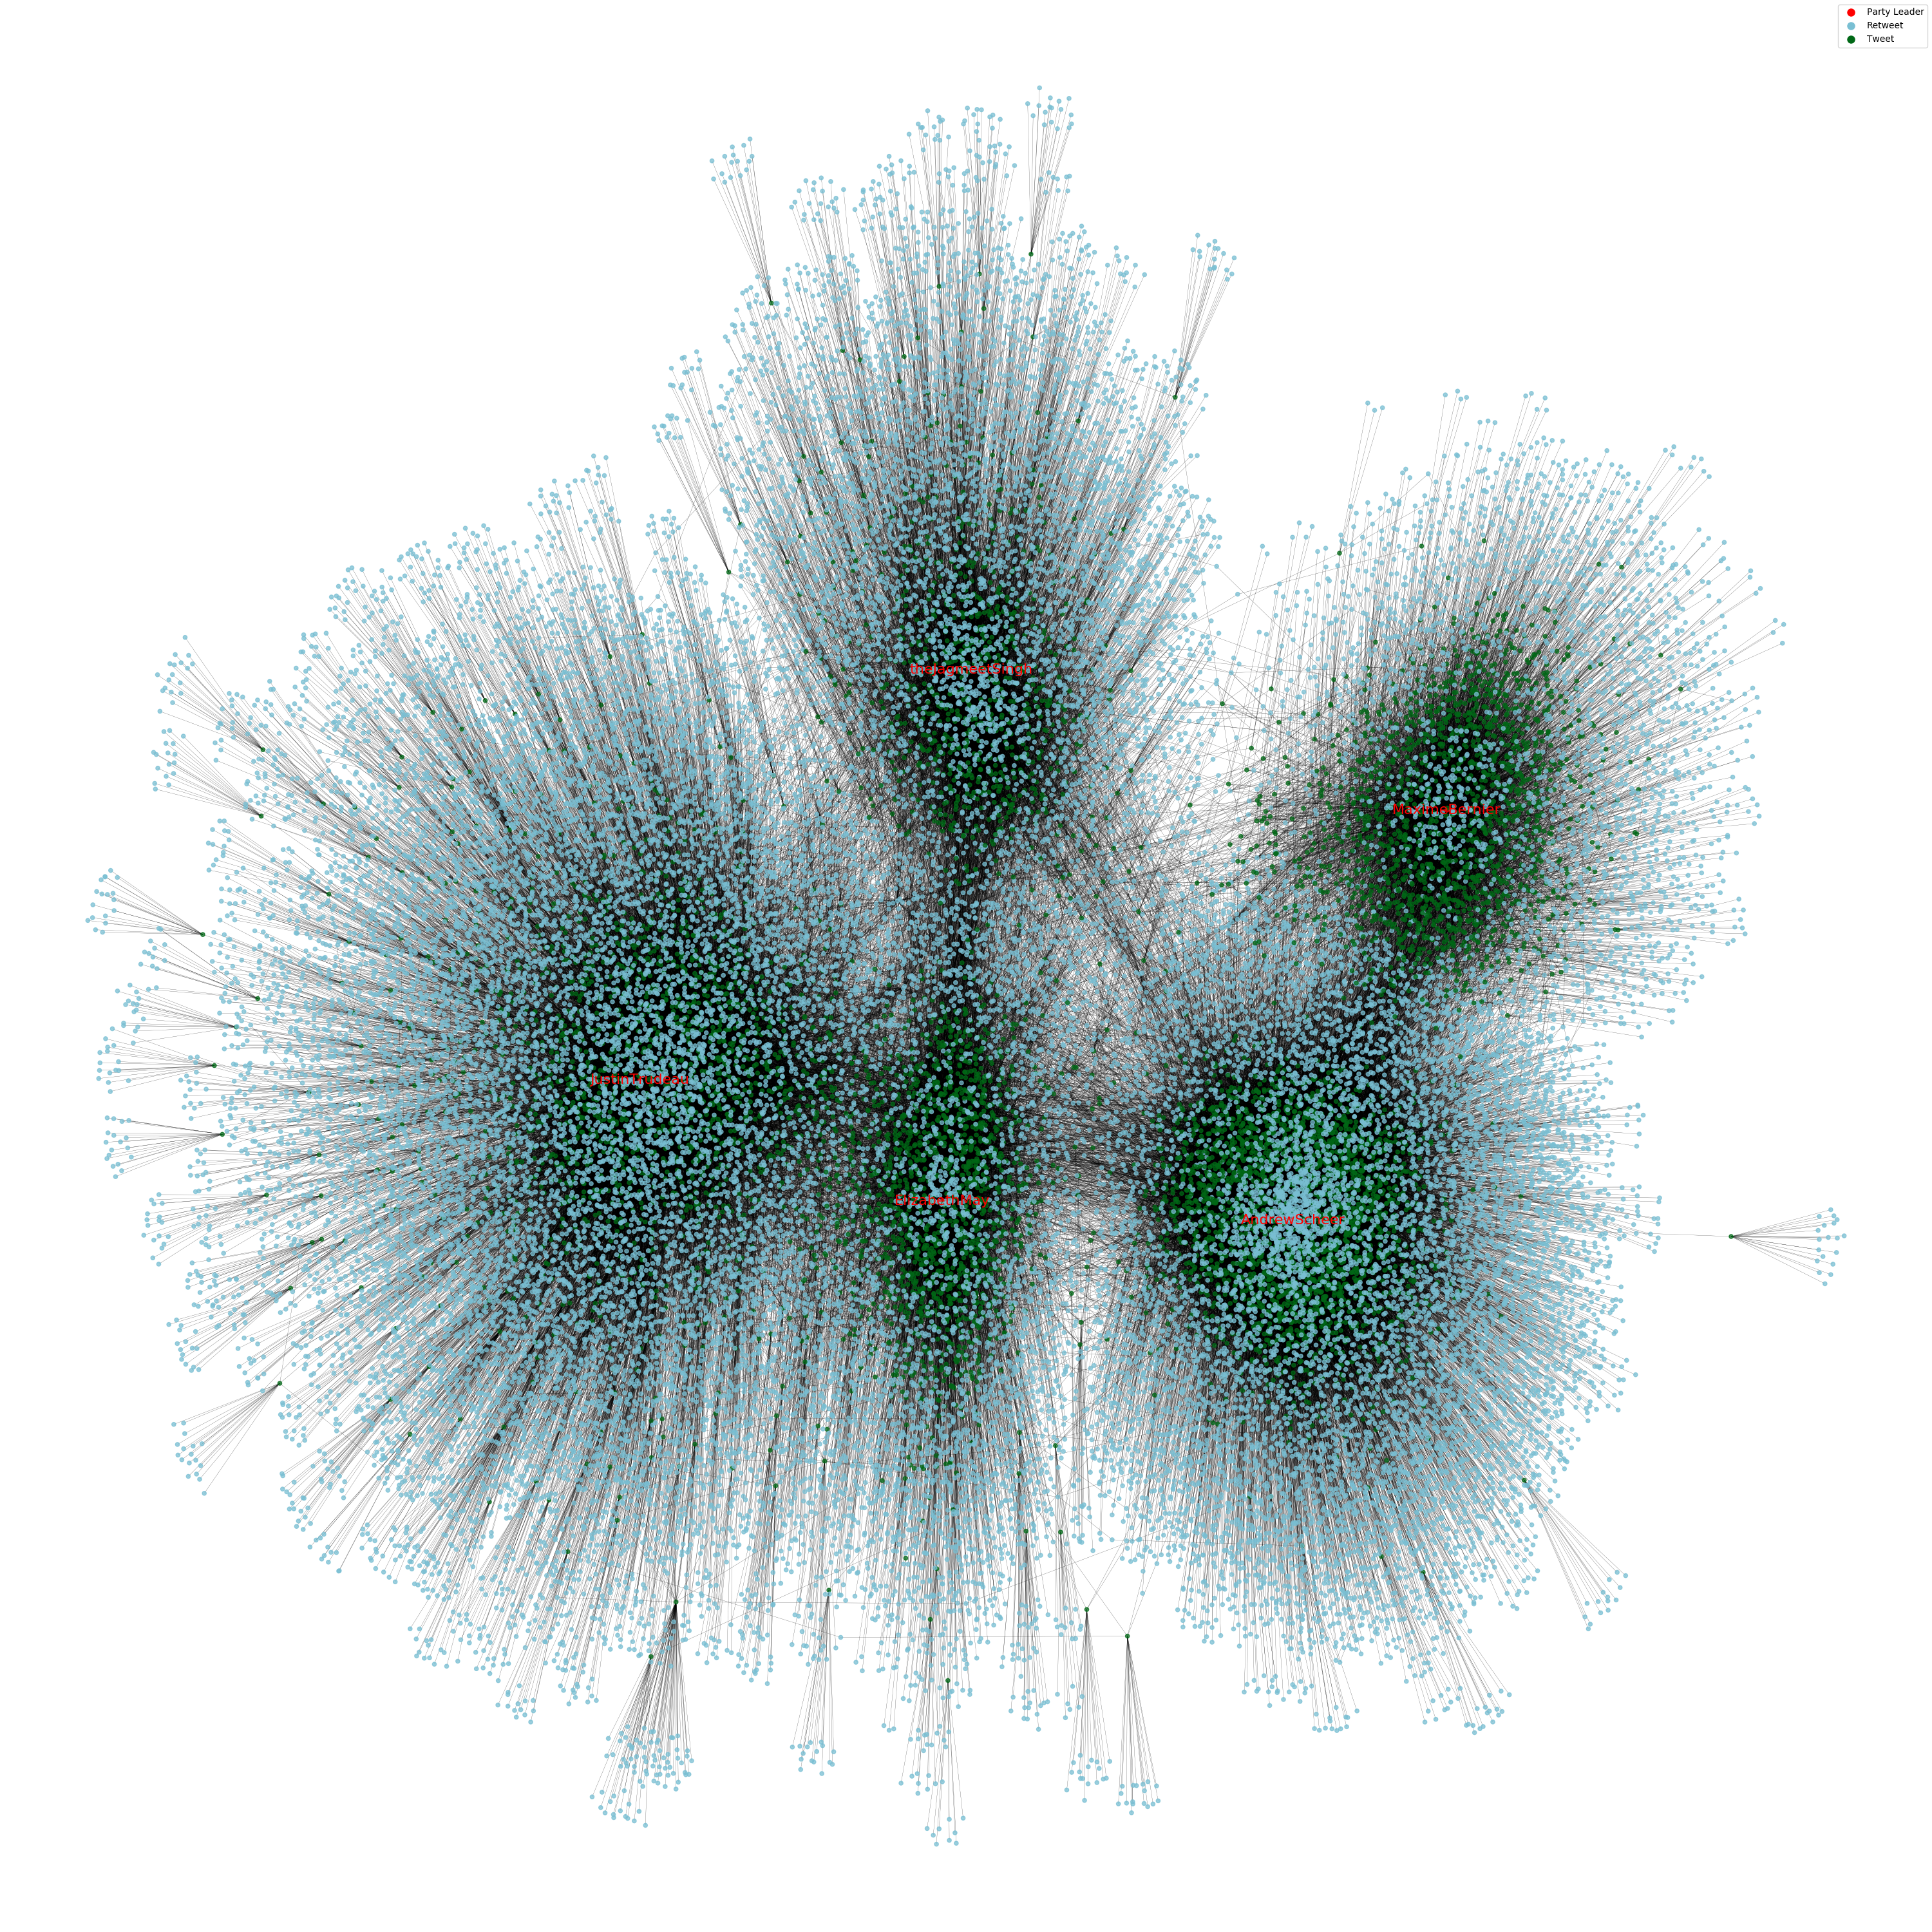
\includegraphics[width=0.75\textwidth]{figures/engagement_graph_no_topics}
  \caption[Full Engagement Graph]{Full Engagement Graph}
  \label{fig:engagement_graph_no_topics}
\end{figure}

\subsection{Topic Modeling}

In order to evaluate the relative importance of various political messages in
driving political engagement on Twitter, all the tweets collected must first be
organized by topic. Given the size of the data, manually coding each label is
inefficient as well as subject to individual biases. As a result, there is a
need for techniques that autonomously organize big, unclassified corpuses of
text. 

Topic modeling methods finds clusters of words that frequently occur together
(topics), connects words with similar meanings, and distinguishes different uses
of words with multiple meanings \cite{alghamdi2015survey}. This is based on the
underlying assumption that a document is concerned with a fixed set of topics,
and that the frequency of words used is indicative of this latent structure
\cite{blei2003latent}. Given that topic extraction approaches based on keywords
are brittle, context specific and are unable to capture emergent topics --
unsupervised machine learning techniques, like the latent Dirichlet allocation
(LDA) developed by Blei et al., are especially useful for autonomous topic
extraction. An LDA model defines two distributions -- one which models topics as
``a distribution over a fixed vocabulary of terms,'' and another which models
documents as a distribution of topics based on the occurrences of words in each
document, the topic distribution per word and the importance of words to each
topic \cite{blei2003latent}. The LDA requires four inputs: the text corpus --
which in this context are the cleaned tweets from all 5 party leaders; $\alpha$
-- which acts as a concentration parameter for how documents are modeled as
topics; $\beta$ -- which acts as a concentration parameter for how topics are
modeled as words; and $k$ -- which is the number of topics to be modeled
\cite{blei2003latent}.

\begin{figure}[h!]
  \centering
  \begin{tabular}{cc}
    \includegraphics[width=0.40\textwidth]{Figures/Coherence_Surface_k=4} &
    \includegraphics[width=0.40\textwidth]{Figures/Coherence_Surface_k=5} \\
  (a) $k=4$ & (b) $k=5$ \\[6pt]
    \includegraphics[width=0.40\textwidth]{Figures/Coherence_Surface_k=6} &
    \includegraphics[width=0.40\textwidth]{Figures/Coherence_Surface_k=7} \\
  (c) $k=6$ & (d) $k=7$ \\[6pt]
  \end{tabular}
  \caption[LDA Parameter Sweep Results]{LDA Parameter Sweep Results}
  \label{fig:lda_param_sweep}
\end{figure}

By performing a parameter sweep, where $\alpha$ and $\beta$ lie on the interval
$[0, 1]$ with increments of 0.05, and $k$ ranges between $4$ and $7$, various
LDAs were exposed to the entire corpus of Tweets and then evaluated using $c\_v$
coherence. Figure \ref{fig:lda_param_sweep} shows, for each $k$ value, the $c\_v$ coherence as a
function of different combinations of $\alpha$ and $\beta$. The most performant
model had a $k$ value of 7, $\alpha$ of 0.31 and $\beta$ of 0.81 and a $c\_v$
coherence score of 0.48. By labelling each tweet as the maximum probability
value in its topic mixture, each tweet was assigned a single topic. The word
clouds for each topic are described in figure \ref{fig:topic_word_clouds}.

\begin{figure}[h!]
    \centering
    \begin{tabular}{cccc}
    \includegraphics[width=0.25\textwidth]{Figures/topic_1_wordcloud} &
    \includegraphics[width=0.25\textwidth]{Figures/topic_2_wordcloud} &
    \includegraphics[width=0.25\textwidth]{Figures/topic_3_wordcloud} &
    \includegraphics[width=0.25\textwidth]{Figures/topic_4_wordcloud} \\
    (a) Topic 1 & (b) Topic 2 & (c) Topic 3 & (d) Topic 4 \\[6pt]
    \includegraphics[width=0.25\textwidth]{Figures/topic_5_wordcloud} &
    \includegraphics[width=0.25\textwidth]{Figures/topic_6_wordcloud} &
    \includegraphics[width=0.25\textwidth]{Figures/topic_7_wordcloud} \\
    (e) Topic 5 & (f) Topic 6 & (g) Topic 7 \\[6pt]
    \end{tabular}
    \caption[LDA Topic Word Clouds]{LDA Topic Word Clouds}
    \label{fig:topic_word_clouds}
\end{figure}

Topic 1 pertained to campaign messages, rallies and logistics – and makes up
8.2\% of all tweets. Topic 2 contains tweets regarding a carbon tax, pipelines
and the economy – and makes up 16.3\% of all tweets. Topic 3 contains tweets
about the SNC Lavalin affair, a scandal that plagued Justin Trudeau, and tweets
about corruption – making up 18\% of all tweets. Topic 4 is predominantly tweets
appealing to the middle-class and economy – and is 29.7\% of all tweets. Topic 5
contains celebratory messages about the campaign, as well as tweets regarding
national holidays and days of remembrance – and make up 15\% of all tweets.
Topic 6 is made up of tweets about immigration, diversity and free speech – and
makes up 11.5\% of all tweets. Finally, Topic 7 contains tweets regarding
healthcare, abortion and pharmacare – and makes up 1\% of all tweets. The
magnitude of how many tweets were assigned to each topic is shown in Figure
\ref{fig:topic_distribution}.

\begin{figure}[h!]
  \centering
  \begin{tabular}{cc}
    \includegraphics[width=0.40\textwidth]{Figures/topic_distribution} &
    \includegraphics[width=0.60\textwidth]{Figures/grouped_bar_by_pl_topic} \\
  (a) Topic Breakdown & (b) Number of Tweets per Topic by Party Leader \\[6pt]
  \end{tabular}
  \caption[LDA Topic Distribution]{LDA Topic Distribution}
  \label{fig:topic_distribution}
\end{figure}

As can be seen by part (b) of Figure \ref{fig:topic_distribution} -- while Topic
6, Tweets pertaining to diversity and immigration, only made up 11.5\% of all
Tweets they made up the majority of Maxime Bernier -- the leader of the newly
founded, populist People's Party of Canada -- Tweets. This signals an attempt on
his part to bring these topics to the forefront of the debate despite few other
party leader's broaching the topic. Additionally, Andrew Scheer and Elizabeth
May's campaigns relied heavily on Topic 3, the SNC Lavalin affair, with a
disproportionate number of Tweets aimed at Justin Trudeau's handling of the
affair. Finally, it can be noted that Maxime Bernier and Andrew Scheer also had
a disproportionate number of Tweets pertaining to Topic 2 -- rebutting Justin
Trudeau's plan to implement a carbon tax, and arguing for greater access to
Alberta's Oil Sands. While an initial assumption may be that each party tailors
such messages to maximize engagement, that remains to be seen without a more
rigorous analysis of how different segments or the electorate as a whole engaged
with each category of message. By assigning each Tweet vertex to a topic and
then coloring the Tweet vertices accordingly, the full engagement graph (Figure
\ref{fig:engagement_graph}) for online political content is complete and ready
for analysis. 

\begin{figure}[h!]
  \centering
  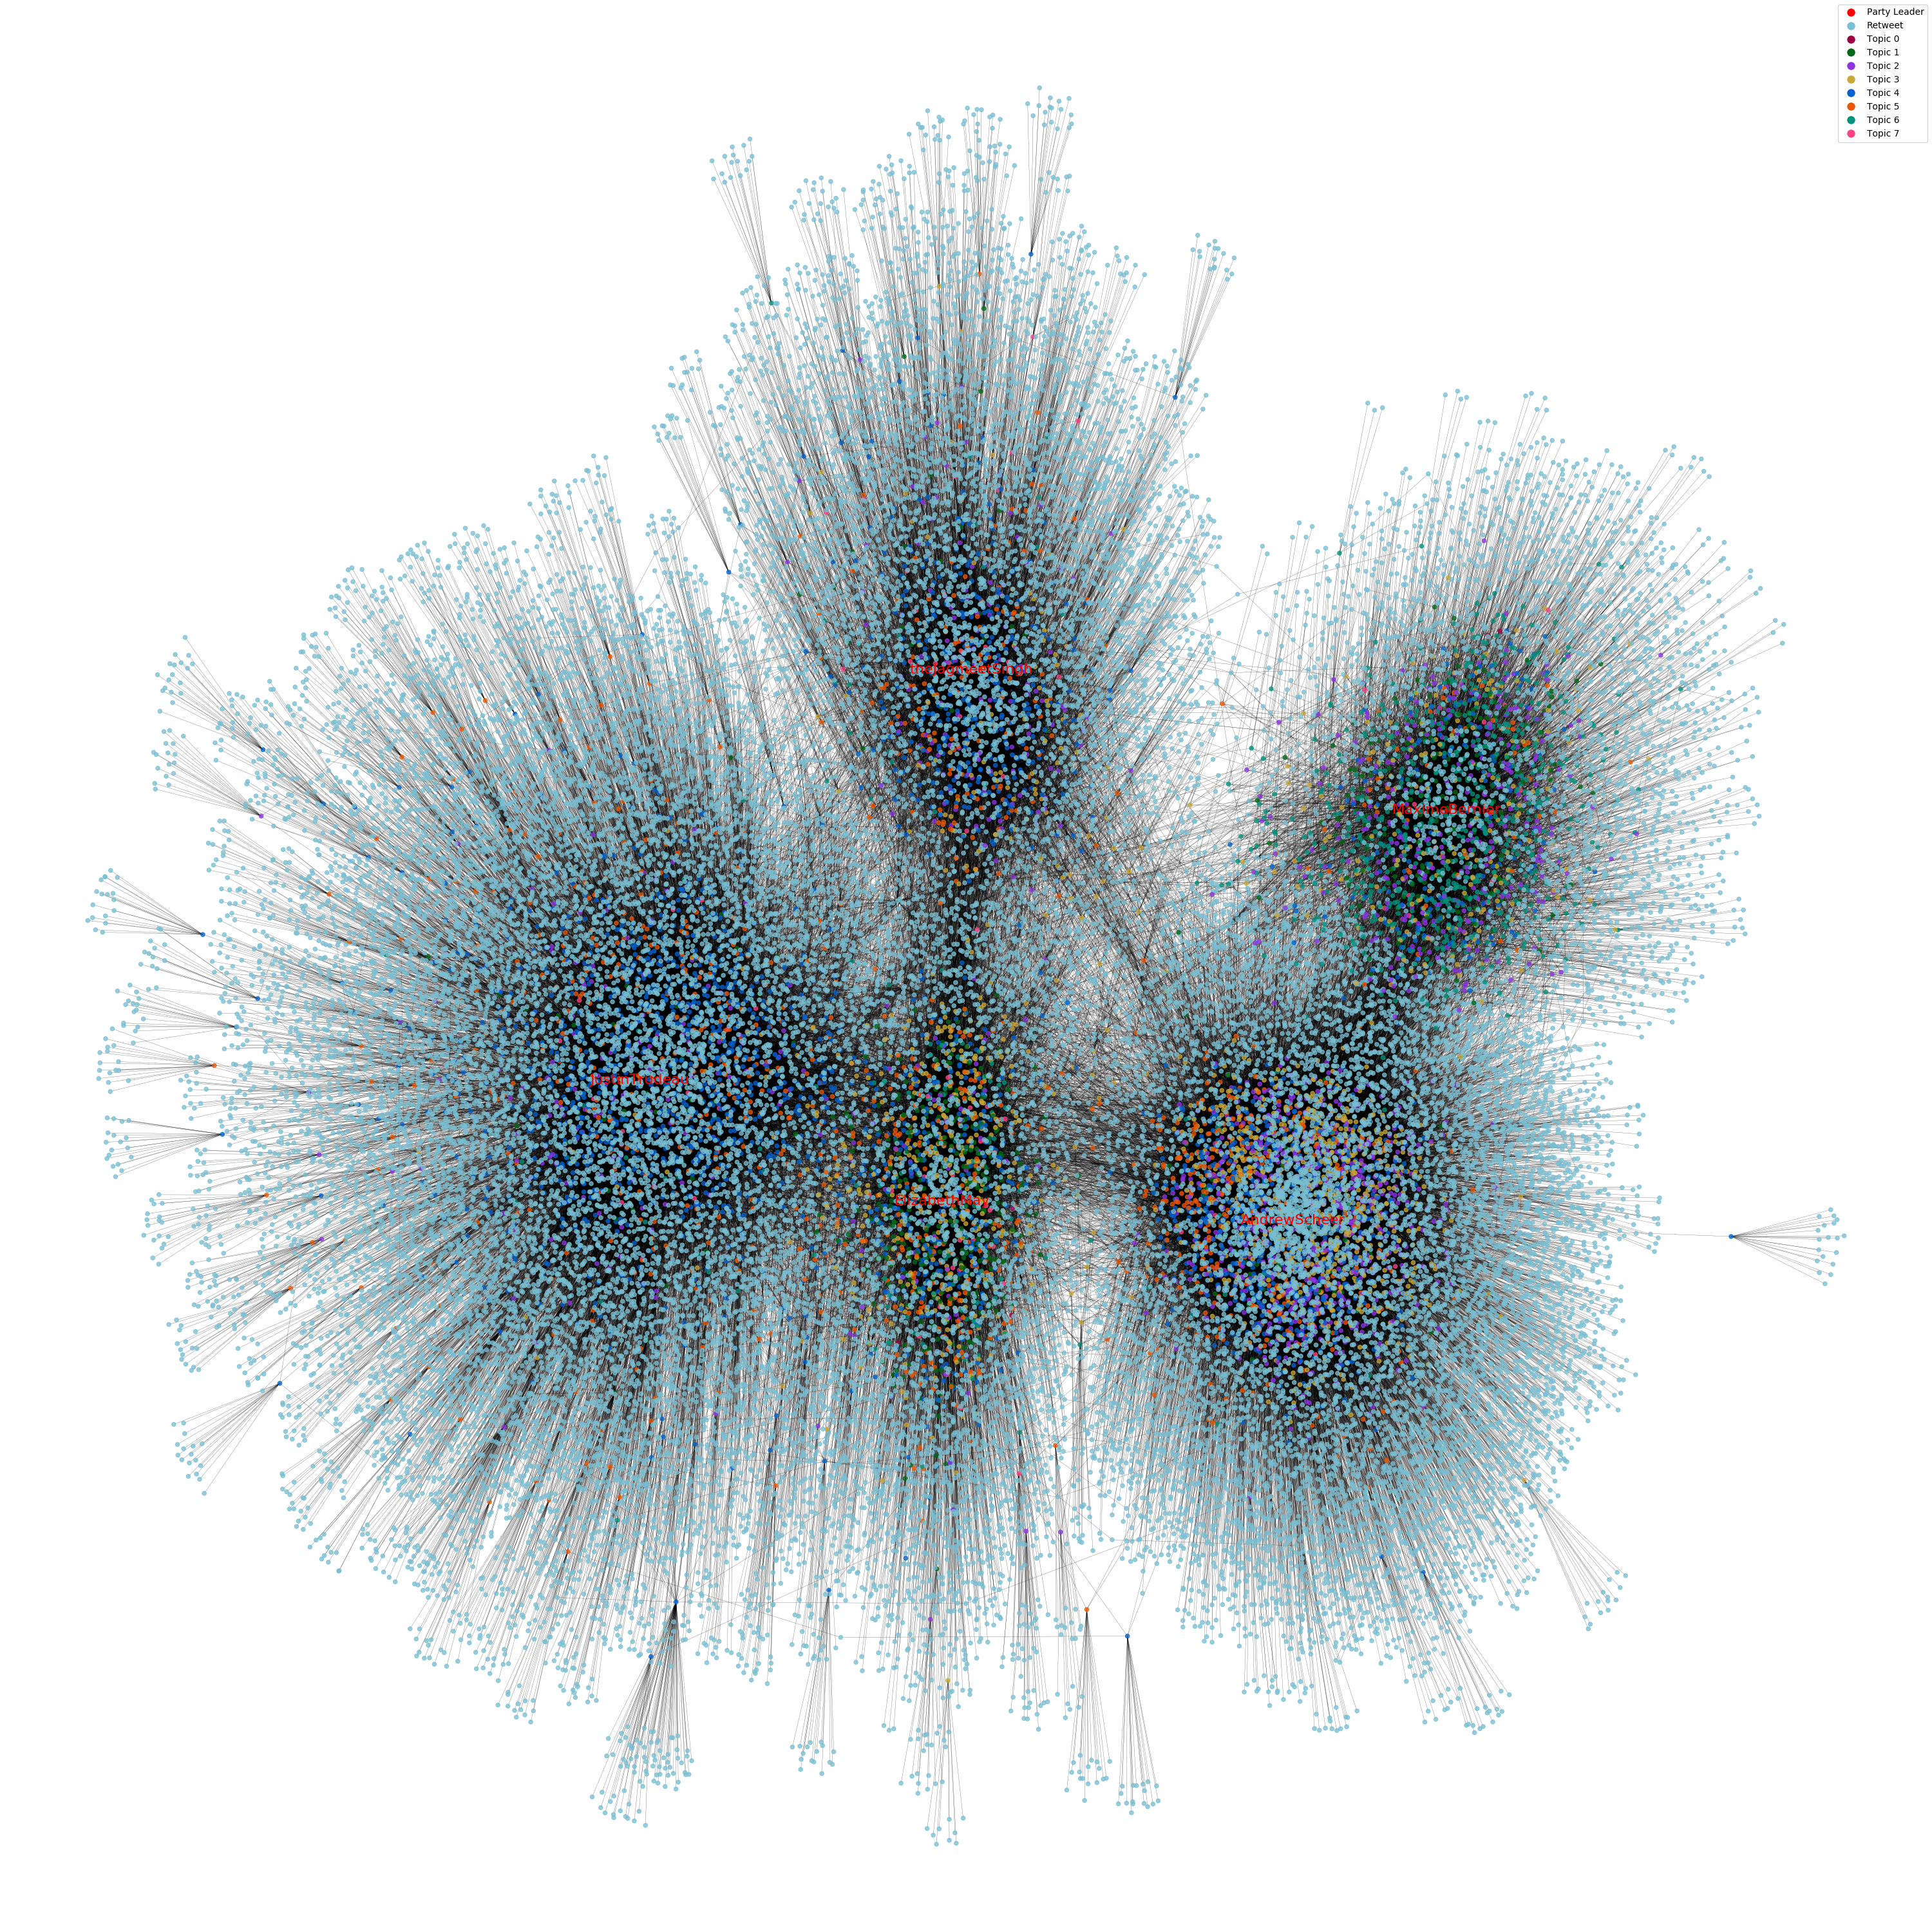
\includegraphics[width=0.75\textwidth]{figures/engagement_graph}
  \caption[Full Engagement Graph]{Full Engagement Graph With Tweet Vertices Colored By Topic}
  \label{fig:engagement_graph}
\end{figure}

\subsection{Topic Centrality}

\subsubsection{Eigenvector Centrality}

\subsubsection{Total Network Topic Centrality}

\subsubsection{Party Leader Topic Centrality}

\section{Results}

\subsection{Topic Saliency}

\subsection{Total Network Topic Centrality}

\subsection{Party Leader Topic Centrality}

\section{Discussion}

% RELATE BACK TO PUTNAM -> Talk about how bridging topics != hunky dory kind of
% discourse. Things can bridge party divides in toxic ways.

\bibliographystyle{nws}
\bibliography{bibliography}

\label{lastpage}

\end{document}

% end of NWSegui.tex